\documentclass{beamer}

\useoutertheme[subsection=false]{miniframes}
\usecolortheme{beaver}
\setbeamertemplate{navigation symbols}{}
\setbeamertemplate{footline}{}
\usepackage{graphicx}
\usepackage{url}
\usepackage{datetime}
\usepackage{tikz-cd}
\newcommand{\lectureDate}{\formatdate{20}{11}{2018}}

\setbeamertemplate{caption}
{\raggedright\insertcaption\par}
\title{MATH211: Linear Methods I}
\author{Matthew Burke}
\date{\lectureDate}
\begin{document}

\frame{\titlepage}

\begin{frame}{Lecture on \lectureDate}
  \tableofcontents
\end{frame}

\section*{Last time}
\label{sec:Last-time}

\begin{frame}{Summary of previous work}
\begin{itemize}
	\item $i^2=-1$
	\begin{itemize}
		\item $(a+bi)+(c+di) = (a+c)+(b+d)i$
		\item $(a+bi)(c+di) = (ac -bd)+(ad+bc)i$
	\end{itemize}\vfill
	\item graphical interpretation
	\begin{align*}
		a+bi &\leftrightarrow (a, b)\\
		\mathbb{C} &\leftrightarrow \mathbb{R}^2
	\end{align*}\vfill
	\item polar form
	\begin{equation*}
		a+ib \leftrightarrow Re^{i\theta}
	\end{equation*}
	where $R$ is the \emph{modulus} and $\theta$ the \emph{angle}.
\end{itemize}
\end{frame}

\section{Examples}

\begin{frame}{Examples}
\begin{example}
Convert the following to polar form:-
\begin{itemize}
	\item $-2+2\sqrt{3}i$ % ANS: 4e^{i*2*pi/3}
	\item $3i$ % ANS: 3e^{i*pi/2}
	\item $-1-i$ % ANS: sqrt{2}e^{i*5*pi/4}
	\item $\sqrt{3}+3i$ % ANS: 2*sqrt(3)e^{i*pi/3}
\end{itemize}
\end{example}
\begin{example}
Convert the following to standard form:-
\begin{itemize}
	\item $2e^{\frac{2\pi i}{3}}$ % ANS: -1+sqrt(3)i
	\item $3e^{-i\pi}$ % ANS: -3
	\item $2e^{\frac{3i\pi}{4}}$ % ANS: -sqrt{2}=sqrt{2}i
\end{itemize}
\end{example}
\end{frame}

\section{Multiplication}

\begin{frame}
\begin{beamercolorbox}[sep=12pt,center]{part title}
\usebeamerfont{section title}
\insertsection\par
\end{beamercolorbox}
\end{frame}

\begin{frame}{Multiplication using polar form}
If $z=Re^{i\theta}$ and $w=Qe^{i\phi}$ then
\begin{align*}
zw&=Re^{i\theta}Qe^{i\phi}\\
 &= (RQ)e^{i(\theta+\phi)}
\end{align*}\vfill
{\bf Slogan:} To multiply two complex numbers we multiply the moduli and add the angles.\vfill
\end{frame}

\begin{frame}{Powers using polar form}
	\begin{theorem}[De Moivre Theorem]
	\begin{equation*}
	(\cos\theta+i\sin\theta)^n = (e^{i\theta})^n = e^{in\theta} = \cos(n\theta)+i\sin(n\theta)
	\end{equation*}
	\end{theorem}
\end{frame}

\begin{frame}{Questions?}
Questions?
\end{frame}

\begin{frame}{Examples}
\begin{example}
Express $(1-i)^6(\sqrt{3}+i)^3$ in the form $a+bi$. % ANS: -64
\end{example}
\begin{example}
Express $(\frac{1}{2}-\frac{\sqrt{3}}{2}i)^{17}$ in the form $a+bi$. % ANS: 1/2 + (sqrt{3}/2)i
\end{example}
\end{frame}

\section{Complex roots}

\begin{frame}
\begin{beamercolorbox}[sep=12pt,center]{part title}
\usebeamerfont{section title}
\insertsection\par
\end{beamercolorbox}
\end{frame}

\begin{frame}{Principal roots}
If $w = Re^{i\theta}$ then one solution to the equation
\begin{equation*}
z^n = w
\end{equation*}
is 
\begin{equation*}
z = \sqrt[n]{R}\cdot e^{\frac{i\theta}{n}}
\end{equation*}
although there will in fact be $n-1$ more solutions.
\end{frame}

\begin{frame}{Square roots}
\begin{columns}
\column{0.5\textwidth}
% 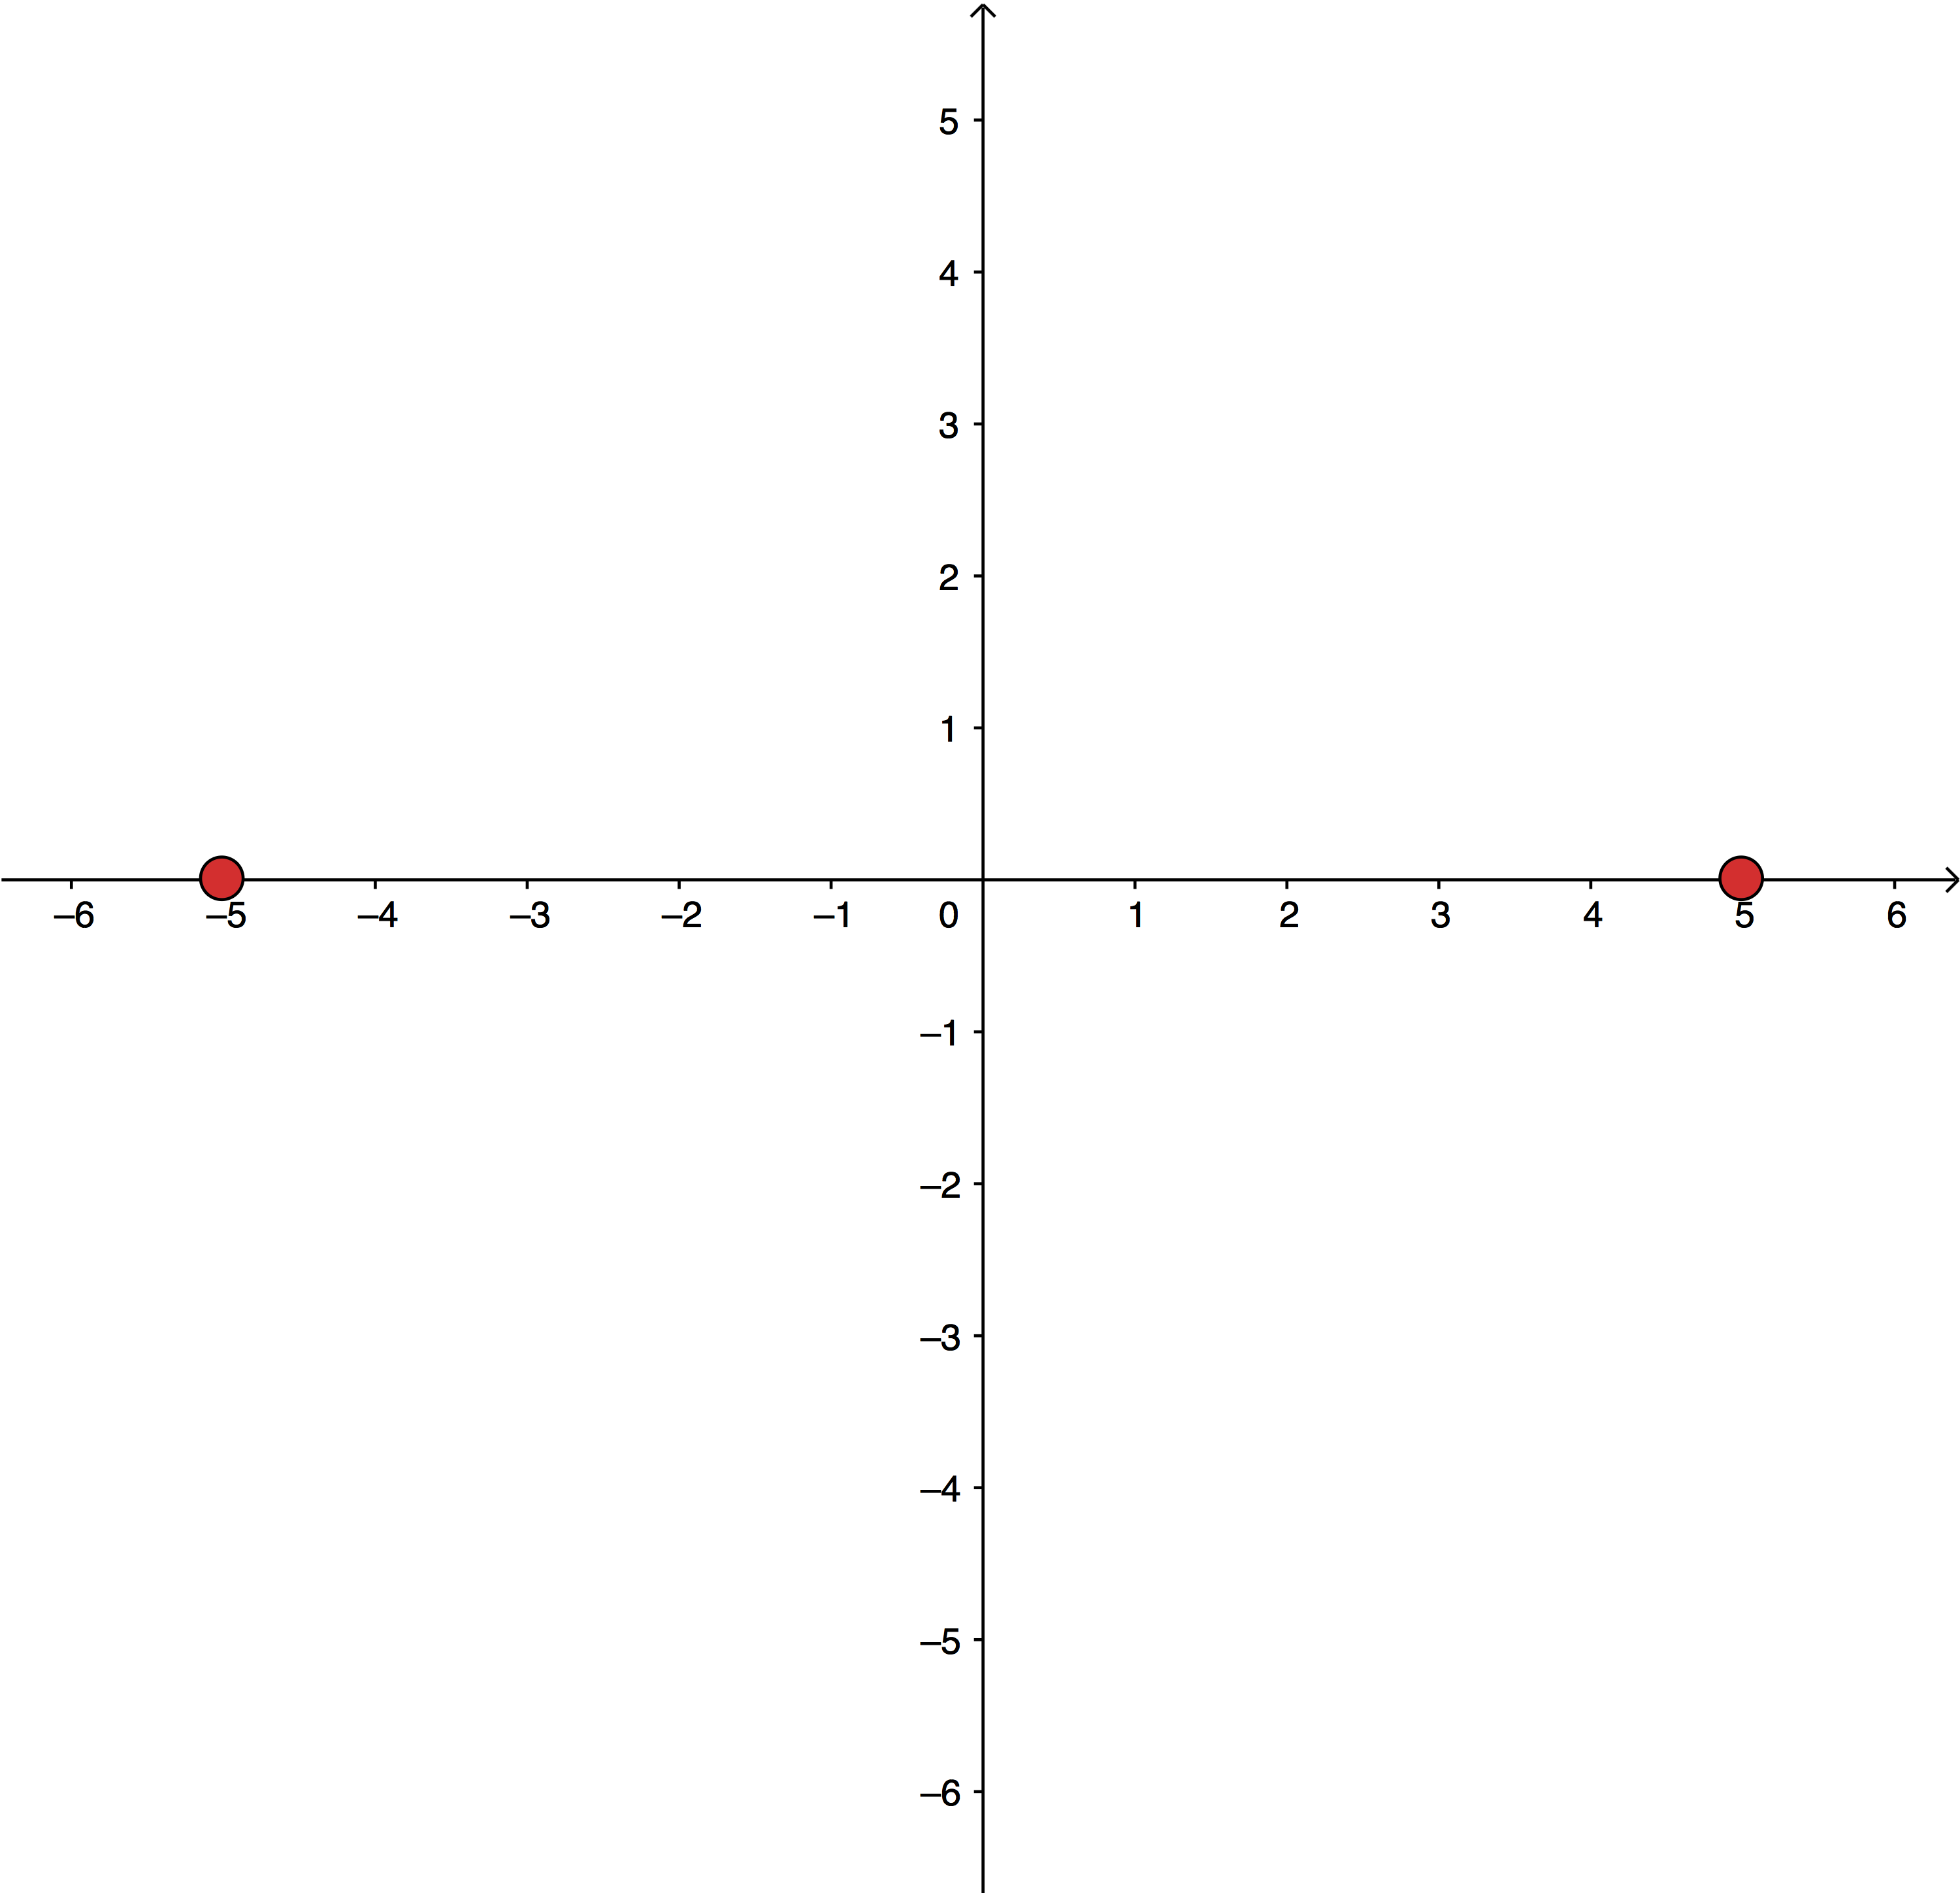
\includegraphics[scale=0.4]{root-25.png}
\column{0.4\textwidth}
The solutions to
\begin{equation*}
	z^2 = 25
\end{equation*}
are
\begin{equation*}
z=+5\text{ and } z=-5
\end{equation*}
\end{columns}
\end{frame}

\begin{frame}{Square roots}
\begin{columns}
\column{0.5\textwidth}
% 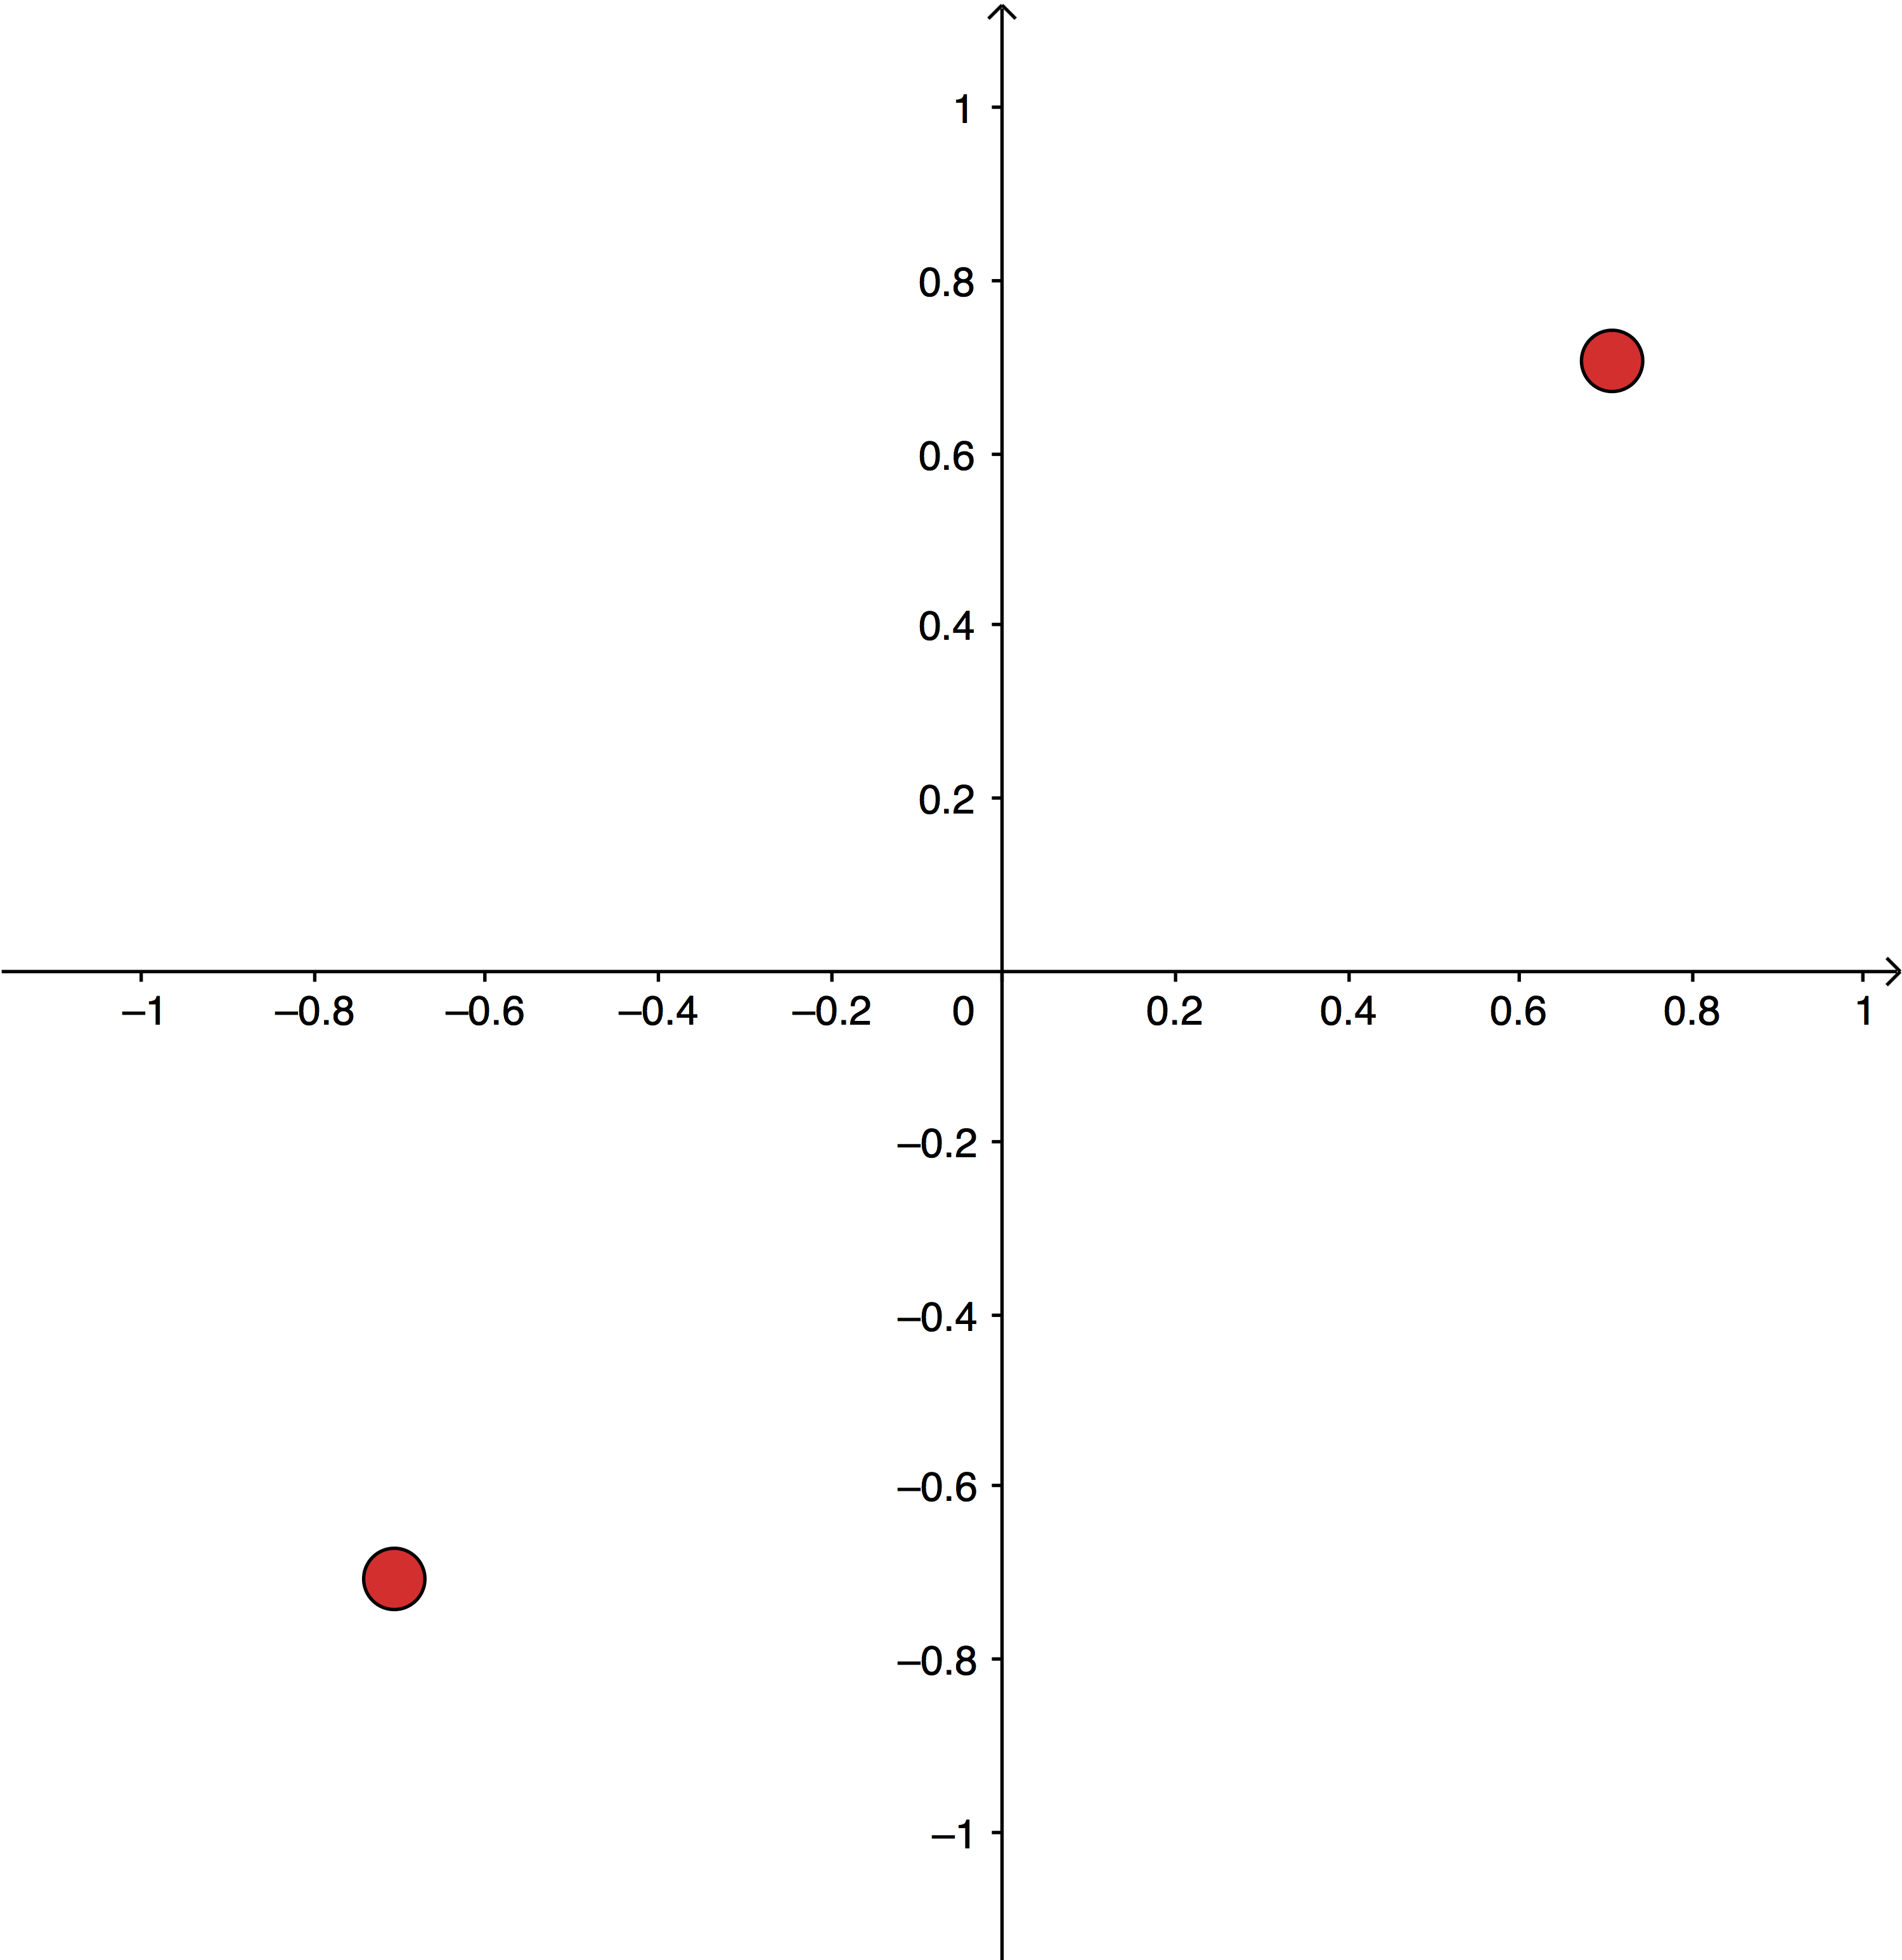
\includegraphics[scale=2.8]{root-i.png}
\column{0.4\textwidth}
The solutions to
\begin{equation*}
	z^2 = i
\end{equation*}
are
\begin{equation*}
z=e^{\frac{\pi}{4}}\text{ and } z=e^{\frac{-3\pi i}{4}}
\end{equation*}
\end{columns}
\end{frame}

\begin{frame}{Square roots}
In general if $w = Re^{i\theta}$ then all of
\begin{equation*}
\sqrt{R}e^{i\left(\frac{\theta}{2}+k\pi\right)}
\end{equation*}
will be square roots of $w$ because
\begin{equation*}
\left(\sqrt{R}e^{i\left(\frac{\theta}{2}+k\pi\right)}\right)^2 = Re^{i\left(\theta+2k\pi\right)} = Re^{i\theta}
\end{equation*}
and then we need to find the values of 
\begin{equation*}
\frac{\theta}{2}+k\pi
\end{equation*}
that are between $-\pi$ and $+\pi$.
\end{frame}

\begin{frame}{Questions?}
Questions?
\end{frame}

\begin{frame}{Examples}
\begin{example}
Find all solutions to the following equations:
\begin{itemize}
	\item $z^2 = 25$. % ANS: -5 and +5
	\item Find all solutions to $z^2 = -1$ % ANS: i and -i
	\item Find all solutions to $z^2 = e^{\frac{i\pi}{4}}$ % ANS: e^{i*pi/8} and e^{-7*i*pi/8}
	\item Find all solutions to $z^3 = i$. (Write in Cartesian form.) % ANS: sqrt(3)/2 + 1/2 i and -i and -sqrt(3)/2 + 1/2 i
	\item Find all solutions to $z^4 = 2(\sqrt{3}i-1)$. (Write in Cartesian form.) % ANS: sqrt{6}/2 + sqrt{2}/2i and + -sqrt{2}/2 +sqrt{6}/2 i and -sqrt{6}/2 - sqrt{2}/2i and  + sqrt{2}/2 -sqrt{6}/2 i
\end{itemize}
\end{example}
\begin{example}
Find all sixth roots of unity.
\end{example}
\end{frame}

\end{document}